54. $(y-2)(x-y)=0\Leftrightarrow\left[\begin{array}{l} y-2=0,\\ x-y=0.\end{array}\right.\Leftrightarrow\left[\begin{array}{l} y=2,\\ y=x.\end{array}\right.$
$$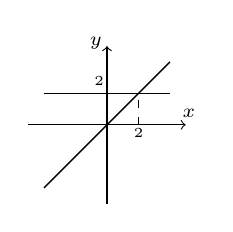
\begin{tikzpicture}[scale=0.2]
\tikzset {line01/.style={line width =0.5pt}}
\tikzset{line02/.style={line width =1pt}}
\tikzset{line03/.style={dashed,line width =0.5pt}}
%\filldraw [black] (0,0) circle (1pt);
\draw [->] (-5,0) -- (5,0);
\draw [->] (0,-5) -- (0,5);
\draw[line01] (-4,2) -- (4,2);
\draw[line01] (-4,-4) -- (4,4);
\draw[line03] (2,0) -- (2,2);
\draw (2,-0.5) node {\tiny $2$};
\draw (-0.5,2.8) node {\tiny $2$};
\draw (5.2,0.7) node {\scriptsize $x$};
\draw (-0.7,5.2) node {\scriptsize $y$};
\end{tikzpicture}$$
